%\documentclass[12pt,fleqn]{article}
%\usepackage[utf8]{inputenc}
%\usepackage{fancyhdr}

\documentclass{article}
\usepackage{graphicx}
\usepackage[a4paper]{geometry} % ensure proper A4 measurements

%\pagestyle{fancy}
%\pagenumbering{gobble}

\author{Christian M\"osl, 01523736}
\title{Aufgabe 2}
\date{}

\begin{document}
\maketitle

\paragraph{}
Es musste ein Auto mit Lineal in xFig nachgezeichnet werden und anschließend um 90 Grad gedreht dargestellt werden.
\vspace{1cm}

\centering
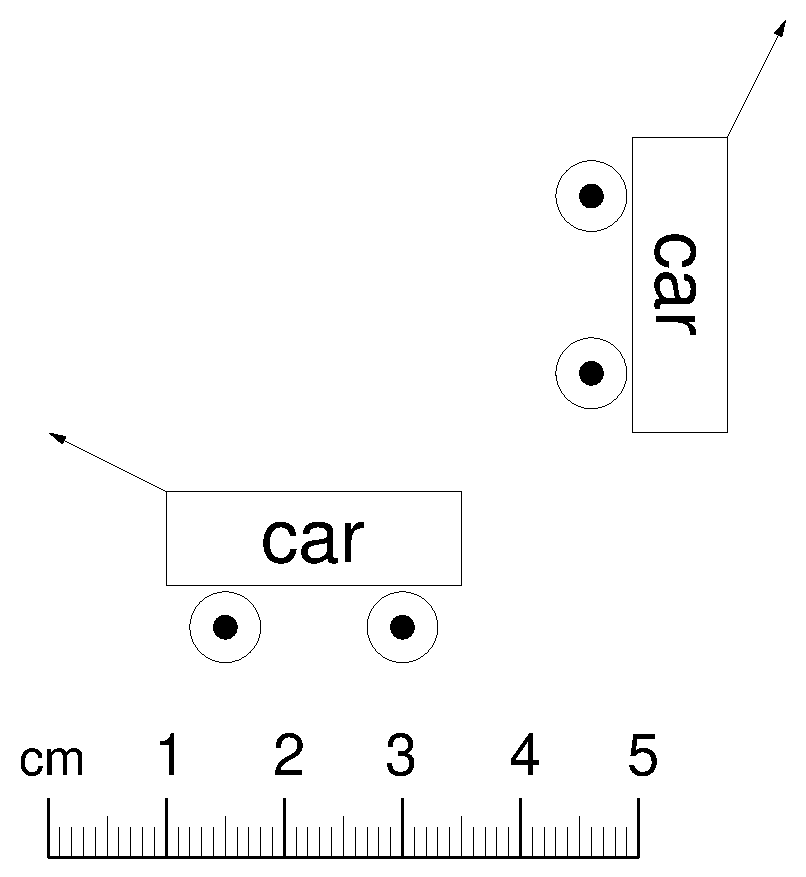
\includegraphics[scale=0.5]{car.eps}
\end{document}
